\section{Translasi Alamat dan Performa}

Pada sistem operasi modern, alamat yang dihasilkan oleh kompilator adalah alamat logis atau \textit{virtual}. Perangkat keras (\textit{MMU}) harus memetakan ini ke alamat fisik di RAM.

\subsection{Virtual to Physical Address}
Proses translasi ini biasanya melibatkan pembagian alamat menjadi \textit{Page Number} dan \textit{Offset}. Kompilator harus memastikan data yang sering diakses bersama-sama berada dalam satu \textit{page} (halaman) yang sama untuk meminimalkan \textit{page fault}.

\subsection{TLB (Translation Lookaside Buffer)}
\textit{TLB} adalah cache khusus di dalam CPU yang menyimpan pemetaan alamat virtual ke fisik yang baru saja digunakan. 
\begin{itemize}
    \item \textbf{TLB Hit}: Alamat fisik ditemukan di TLB, akses sangat cepat.
    \item \textbf{TLB Miss}: CPU harus mencari di tabel halaman (\textit{page table}) di RAM, yang jauh lebih lambat.
\end{itemize}

\subsection{Pentingnya Lokalitas Spasial}
Manajemen memori oleh kompilator (seperti pemilihan \textit{Row-Major order}) sangat krusial karena mendukung \textbf{Lokalitas Spasial}.
\begin{itemize}
    \item Jika elemen array diakses secara berurutan sesuai layout memori, maka data tersebut kemungkinan besar sudah ada di cache CPU dan pemetaan halamannya sudah ada di TLB.
    \item Lompatan alamat yang acak atau besar dapat menyebabkan \textit{TLB Miss} dan \textit{Cache Miss} berulang kali, menurunkan performa program secara drastis meskipun algoritma di tingkat tinggi tampak efisien.
\end{itemize}

\begin{figure}[!htbp]
    \centering
    \adjustbox{max width=0.8\textwidth,center}{%
    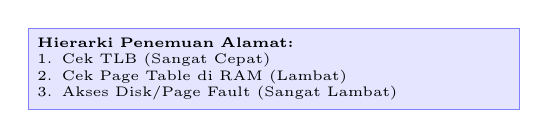
\begin{tikzpicture}[
        seg/.style={rectangle, draw=blue!50, fill=blue!10, text width=6cm, font=\tiny}
    ]
    \node[seg] (tlb) {
        \textbf{Hierarki Penemuan Alamat:}\\
        1. Cek TLB (Sangat Cepat)\\
        2. Cek Page Table di RAM (Lambat)\\
        3. Akses Disk/Page Fault (Sangat Lambat)
    };
    \end{tikzpicture}%
    }
    \caption{Alur Penemuan Alamat Fisik di Perangkat Keras}
\end{figure}
